\documentclass{beamer}
\usepackage[version=4]{mhchem} 
\usepackage{tikz}


\usetheme{Madrid}
\usecolortheme{beaver}

\title{Unit 1}
\subtitle{Motion and Force}
\author{Mr. Maxwell}
\institute{PACS}
\date{\today}


\begin{document}

\frame{\titlepage}

\section{Motion in one and two dimensions}

\begin{frame}
    \frametitle{frame of reference}
    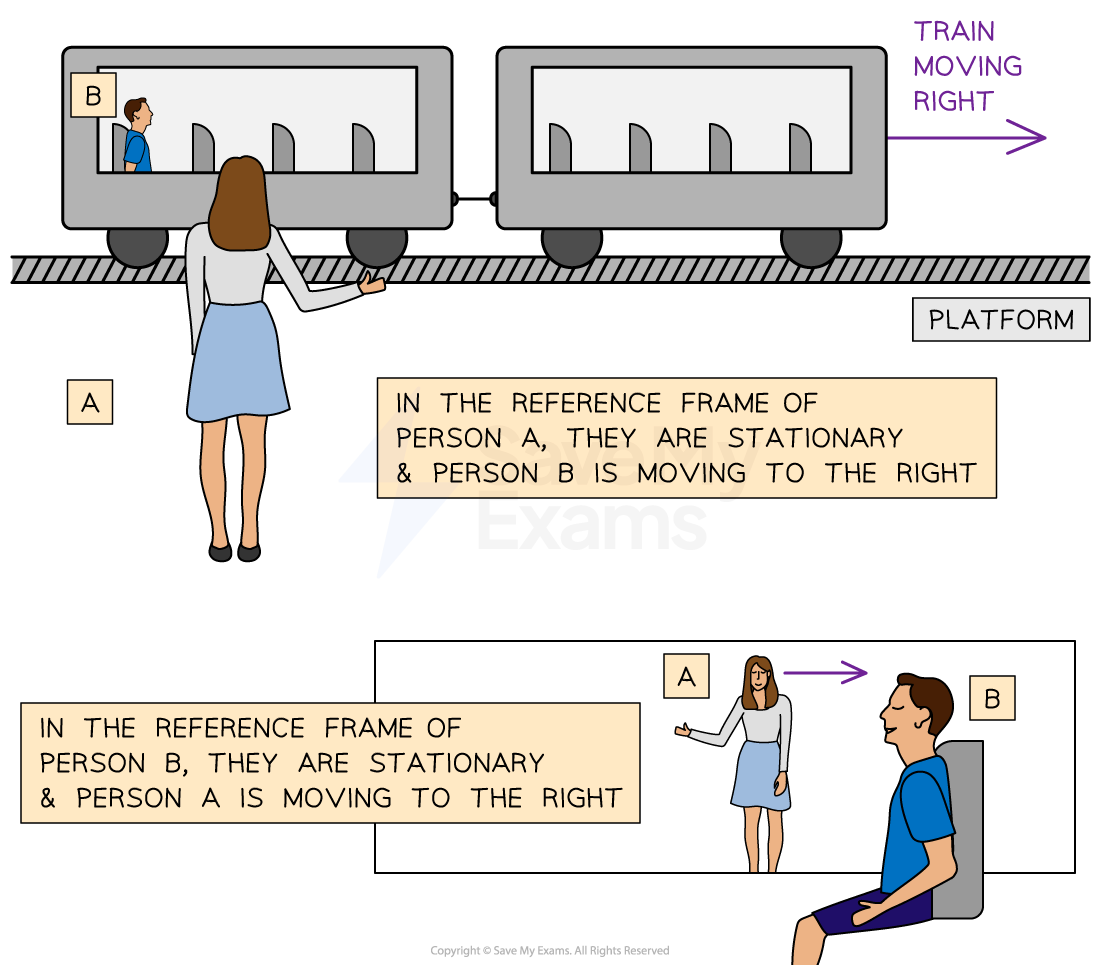
\includegraphics[width=4cm]{../../images/frame_of_reference.png}
    \begin{columns}
        \begin{column}{5cm}
            \onslide a system for specifying the precise location of objects in space and time\\
        \end{column}
        \begin{column}{5cm}
        \pause un sistema para especificar la ubicación precisa de objetos en el espacio y el tiempo
    \end{column}
    \end{columns}


\end{frame}







\end{document}